\documentclass[conference]{IEEEtran}
\IEEEoverridecommandlockouts

\usepackage{cite}
\usepackage{amsmath,amssymb,amsfonts}
\usepackage{algorithmic}
\usepackage{graphicx}
\usepackage{textcomp}
\usepackage{xcolor}
\usepackage{tikz}
\usepackage{multirow}
\usetikzlibrary{positioning}
\usepackage{hyperref}
\usepackage{colortbl}
\usepackage{tabularx}
\usepackage{array}
\usepackage{booktabs}
\usepackage[font=small,labelfont=bf,justification=centering,singlelinecheck=false]{caption}
\usepackage{capt-of}
\usepackage{stfloats}
\usepackage{placeins}
\usepackage{multicol}
\usepackage{float}
\usepackage[hypcap=false]{caption}
\setcounter{dbltopnumber}{3}
\renewcommand{\dbltopfraction}{0.9}
\renewcommand{\dblfloatpagefraction}{0.75}
\setlength{\abovecaptionskip}{4pt}
\setlength{\belowcaptionskip}{4pt}
\newcolumntype{L}[1]{>{\raggedright\arraybackslash}p{#1}}
\newcolumntype{Y}{>{\raggedright\arraybackslash}X}
\def\BibTeX{{\rm B\kern-.05em{\sc i\kern-.025em b}\kern-.08em
    T\kern-.1667em\lower.7ex\hbox{E}\kern-.125emX}}


\begin{document}
\raggedbottom

\title{
Master Thesis Proposal\\
Fault-Tolerant Decentralized Multi-Agent Coordination for Smart Warehouse Inspection Systems with Inventory Anomaly Detection
}


\author{\IEEEauthorblockN{Can Özkan}
\IEEEauthorblockA{\textit{Master of Software Engineering} \\
\textit{Univ. of Europe for Applied Sciences}\\
Potsdam 14469, Germany \\
can.ozkan@ue-germany.de}
}

\maketitle

\begin{abstract}

The modern logistics sector is undergoing a major transformation due to increased e-commerce demands aligned with Industry 5.0, workforce shortages, and the critical need for real-time inventory visibility. However, current warehouse management systems utilizing centralized architectures carry the risk of a Single Point of Failure (SPOF); in dynamic environments, a single robot failure can cause a total operational halt. Such disruptions lead to costly delays affecting industrial efficiency and resulting in significant data losses. The primary goal of this thesis is to develop a fault-tolerant and decentralized multi-agent coordination architecture for smart warehouse environments to enhance system resilience.

The research process will be conducted using Turtlebot3 Waffle platforms within the ROS2 Jazzy and Gazebo Harmonic simulation environments, running on an Ubuntu WSL2 infrastructure. Methodologically, the Nav2 stack and Cartographer SLAM algorithms will be integrated for navigation, while the XGBoost machine learning algorithm, supported by Local Binary Patterns (LBP) feature extraction, will be utilized to detect and classify damaged packages. System performance will be evaluated through a load-balanced task redistribution algorithm under failure scenarios and visualized via a multi-threaded PyQt5 user interface. By providing an end-to-end integration of decentralized fault-tolerance mechanisms with artificial intelligence-based auditing processes, this study aims to minimize operational downtime and maximize inventory reliability.

\end{abstract}

\section{Introduction}

In the era of Industry 4.0 and 5.0, due to increasing demands on e-commerce, workforce shortages, and the need for real-time inventory visibility, the logistics sector is facing significant difficulties\cite{zhang2025autonomous}. Traditional warehouse management systems lack the flexibility and operational efficiency to meet these high demands\cite{zhang2025autonomous}. In this context, unmanned air vehicles' (UAV) integration to warehouse operations, by limiting human intervention, increases the accuracy and speed of stock taking, mapping and auditing processes\cite{pore2026drone}. Especially, the Smart Warehouse concept, by using the synergy of robotic autonomy with cyber-physical systems, is redefining the global supply chain standards \cite{pore2026drone}.

Most current studies in the literature still focus on limited single-UAV systems in simulation environments and cannot sufficiently analyse multi-agent coordination and its challenges \cite{pore2026drone}. One of the biggest limitations of existing systems is that centralised architectures are prone to "single point of failure" (SPOF) risks and are inadequate for providing reliable coordination in complex and dynamic warehouse environments \cite{abro2024synergistic}. Although many studies are based on static environments, in real-world scenarios, when a robotic agent fails, how the mission will continue and how system resilience will be maintained still remain gaps in the literature\cite{abro2024synergistic}. In addition, end-to-end integration of anomaly detection with dynamic task distribution and decentralised coordination solutions is still needed \cite{fourie2025development}.

The aim of this study is to develop a fault-tolerant and decentralized multi-agent coordination architecture for smart warehouse environments in order to increase the efficiency and resilience of the system. The main research questions of this study are:

\begin{enumerate}

    \item How does load-balanced task redistribution among other agents, in the case of one UAV failure, affect the recovery time of the system?

    \item How low can the latency be, and how high can the precision of an XGBoost-based anomaly detection model be in classifying damaged packages in warehouse environments?

    \item To what extent does the increase in the count of agents optimize the total warehouse audit time?

\end{enumerate}

Although the study is inspired by UAV-based warehouse inspection scenarios, the proposed coordination architecture is evaluated through Turtlebot3 robotic proxies in order to focus on coordination behaviour, fault tolerance, and anomaly detection mechanisms rather than flight dynamics. 

This proposed research offers a unique integration model to the literature by combining decentralized fault-tolerant mechanisms with machine learning-based auditing processes. Even though there are similar warehouse simulations using Turtlebot Waffle platforms, these studies generally focus on pick-and-place tasks\cite{leite2024coordination}; autonomous auditing and load-balanced task allocation is still an authentic research field. The results have the potential to reduce robotic downtime and improve inventory anomaly detection reliability. From a practical perspective, the load-balanced task redistribution algorithm developed in this study may optimize resource usage in logistics operations and reduce operational costs. Moreover, the proposed architecture can be extended to UAV-based warehouse inspection systems in future work. In conclusion, this research aims to provide a technical foundation for resilient human-machine collaboration systems within the vision of Industry 5.0.

 
\section{Problem Statement}

The usage of centralized systems in modern warehousing operations causes the whole system to cease in the case of a single robot failure. This condition (SPOF) makes operational continuity impossible. \cite{abro2024synergistic}. In the case of a robotic agent's failure, causing inability to provide task sustainability, costly delays in audit processes and data losses which affect industrial efficiency negatively\cite{arvind2025intelligent}. This situation transforms the need for fault-tolerant autonomous solutions that minimize human intervention while increasing system resilience into a critical industrial necessity.

Existing literature, for the most part, approaches to autonomous cruising and anomaly detection subjects separately, do not offer end-to-end integration where, in case of a failure, tasks are automatically assigned to other robots\cite{zhang2025autonomous}, this detachment can slow down the system's reaction time in dynamic situations such as robot failures. This research aims to fill this gap by offering a decentralized architecture that redistributes the remaining jobs in a load-balanced way among remaining agents when an agent is disabled. The proposed model aims to optimize smart warehouse automation operation efficiency and audit reliability by combining inventory audit processes that are supported by the XGBoost algorithm with ROS2-based fault tolerance mechanisms.

\section{Research Objectives}

\begin{itemize}

    \item \textbf{To design a decentralized architecture} - In order to eliminate the single point of failure (SPOF) risk, design a decentralized multi-agent coordination infrastructure that depends on direct communication between robots, ROS2-based. 

    \item \textbf{To develop a fault-tolerant job distribution algorithm} - In the event of a robot's failure, develop a mechanism that distributes the remaining unfinished tasks (waypoint list) to other active agents in the system in a load-balanced way. 

    \item \textbf{To develop machine learning-based anomaly detection} - Train a highly sensitive XGBoost model that uses feature extraction methods such as LBP and integrate it into a robotic system in order to successfully identify and classify the damaged packages in the warehouse inventory. 

    \item \textbf{To analyze system performance and scalability} - To analyze the error recovery time, total audit efficiency, and anomaly detection accuracy through quantitative data under different robot counts (1,2 and 3 agents) and controlled failure scenarios

    \item \textbf{To develop real-time monitoring infrastructure} - to develop a multi-threaded user interface that is working synchronously with the ROS2 ecosystem that presents robot locations, task completion rates, and system notifications to the operator. 

\end{itemize}

\section{Literature Review}

This study falls into the intersection of job distribution in multi robotic systems, fault-tolerant coordination and machine learning-based warehouse auditing disciplines. Existing studies in the literature are analyzed under three main themes:

\subsection{Distributed Task Allocation in Multi Agent Systems}

Traditional centralized control architectures, in large-scale warehouse operations, contain structural risks such as a single point failure (SPOF) and communication bottlenecks. Contemporary literature proposes distributed frameworks that utilize big data analysis and consensus algorithms in order to overcome these limitations\cite{hayes2026decentralized}. It was observed that dynamic path planning systems supported by multi-agent approaches have increased the operational efficiency and speed for autonomous mobile robots in complex environments\cite{fourie2025development}. However, most of these studies focus on stable system states and keep the sudden agent loss effect in the background.

\subsection{Fault Tolerant and Integrated Coordination Mechanisms}

Integrated models that intertwine task allocation and safe coordination to make robotic systems more resilient in dynamic warehouse environments are being developed\cite{miele2025distributed}. In particular, it has been proven that in redundant systems where the agent count exceeds the task count, iterative consensus algorithms provide operational continuity even in the case of agent failure\cite{govoni2024decentralized}. Network analysis of decentralized fault-tolerant UAV swarm coordination in critical missions demonstrates that decentralized fault-tolerant strategies in complex and unexpected scenarios affect the mission success directly\cite{chandran2024network}.

\subsection{Warehouse Automation, Simulation and Anomaly Detection}

Using ROS and Gazebo ecosystems to test the theoretical algorithms in practical warehouse scenarios has become a standard in the literature. It was observed that, in particular simulations that utilize Turtlebot Waffle platforms, Supervisory Control Theory has provided modular and scalable coordination\cite{leite2024coordination}. On the side of the inventory auditing, it is underlined that cyber-physical systems and Internet of Things (IoT) frameworks combined with machine learning increase the stock accuracy\cite{arvind2025intelligent}. Even though visual processing-based shelf status recognition studies reach high precision rates\cite{zhang2025autonomous}, the real-time and end-to-end integration of anomaly detection processes with autonomous task allocation algorithms still remains as a gap in the literature.

\clearpage
\onecolumn
\makeatletter
\setlength{\@fptop}{0pt}
\makeatother
\setlength{\abovecaptionskip}{0pt}
\setlength{\belowcaptionskip}{0pt}
 
% ----------------------------------------------------------
% TABLO 1 
% ----------------------------------------------------------
\begin{table}[!t]
\centering
\footnotesize
\setlength{\tabcolsep}{4pt}
\renewcommand{\arraystretch}{1.05}
\caption{COMPARATIVE ANALYSIS OF EXISTING LITERATURE ON MULTI-AGENT COORDINATION, FAULT TOLERANCE AND ANOMALY DETECTION IN SMART WAREHOUSING}
\label{LitRevTable_1}
\begin{tabularx}{\linewidth}{@{}L{0.7cm}L{2.0cm}L{2.0cm}L{3.6cm}L{3.8cm}Y@{}}
\toprule
\textbf{Ref \& Year} &
  \textbf{Author \& Title} &
  \textbf{Dataset / Environment} &
  \textbf{Method(s)} &
  \textbf{Key Results} &
  \textbf{Contributions vs. Gaps} \\ \midrule
\cite{zhang2025autonomous} 2025 &
  Zhang \& Abellera -- Autonomous mobile robotics in smart warehousing &
  Industrial smart warehouse; real deployment + digital twin &
  CPS architecture; AMR fleet coordination; distributed task allocation; dynamic path planning; edge-cloud analytics &
  42\% faster order fulfillment; 35\% lower inventory cost; 89\% real-time stock accuracy; 99.2\% uptime; handled 3x peak demand &
  Contribution: Integrated CPS-AMR-digital twin framework with real-world validation.\newline Gap: Limited conflict/deadlock analysis; robot/sensor failure recovery not explicitly modeled. \\ \midrule
\cite{pore2026drone} 2026 &
  Pore et al. -- Drone-Enabled Practices in Modern Warehouse Management &
  118 studies (453 screened); mostly static and simulation-based; limited real deployments &
  Systematic review; taxonomy of applications/platforms; single vs multi-UAV; simulation vs real-time; AI/RFID/LiDAR/IoT stacks &
  Inventory management: 52\%; layout optimization: 19\%; security: 13\%; picking/transport: 10\%; maintenance: 5\%; up to 40\% inventory reduction and 91--99\% QR/RFID accuracy in reported cases &
  Contribution: Consolidates literature into a clear taxonomy and maturity map.\newline Gap: Strong single-agent and simulation bias; limited validated multi-agent coordination and real fault-tolerance evidence. \\ \midrule
\cite{abro2024synergistic} 2024 &
  Abro, Ali \& Masood -- Synergistic UAV Motion &
  Survey of simulation-heavy studies with limited real-world UAV validation (2008--2024) &
  Systematic review; bio-inspired models; decentralized control; MPC, PSO, ACO, GA, and RL methods; formation and path planning &
  Reviews 60+ studies over $\sim$16 years; reports scalability/resilience trends but no unified benchmark due to heterogeneous evaluations &
  Contribution: Structured synthesis linking collective-motion theory to modern multi-agent control.\newline Gap: Limited large-scale real validation and no systematic comparison of failure-recovery strategies. \\ \midrule
\cite{fourie2025development} 2025 &
  Fourie, Louw \& Bitsch -- Development of a Dynamic Path Planning System &
  Simulated FMS and logistics learning factory; 30x30 m grid-based environments; up to 10 AMRs; realistic Industry 4.0 disturbance scenarios &
  Decentralized MAS with hybrid GA cell decomposition; multi-objective fitness (length, smoothness, overlap); IEP-based predictive collision avoidance via blackboard &
  Zero deadlocks / collisions to 9 AMRs; 1 collision per 1000 trials at 10 AMRs; near-optimal path length; smoother than Dijkstra/RL; runtime $\sim$2-17.5s; robust replanning under obstacles, human interference, and failures &
  Contribution: Integrates hybrid GA path planning with decentralized MAS \& IEP, optimizing path overlap and demonstrating robust multi-agent coordination \& disturbance handling in realistic FMS scenarios. \newline Gap: Fault tolerance is limited to reactive replanning (no formal recovery for communication loss or agent failure); coordination scalability degrades under extreme congestion and lacks hierarchical or clustered multi-agent coordination for large fleets.\\ \midrule
  \cite{leite2024coordination} 2024 & Leite, E.F. -- Coordination of Multi-Agent Systems & Simulated warehouse automation using ROS2 Humble and Gazebo Classic with TurtleBot Waffle Pi robots, pick-\&-place tasks, variable robot count (1 vs. 4), 10min simulations & Scalable Supervisory Control Theory (SSCT); Discrete Event Systems modeling; relabeling-based scalable supervisors; ROS2 node-based supervisor-plant integration; Gazebo simulation; Nav2 navigation & With four robots, bounded input/output demand remains stable while single-robot case shows unbounded demand growth; average task completion time $\sim$0.8-1.0 min (1 robot) vs. $\sim$0.9-1.2 min (4 robots); parallel tasks increase from max. 1 to about 3-4 concurrent tasks; supervisor state reduction from 492 states and 1484 transitions (monolithic SCT, 2 robots/2 storage) to 8-31 states and 14-98 transitions (SSCT/local) enabling scalability & Contribution: Demonstrates practical SSCT deployment for multi-agent coordination, showing deadlock-free operation, improved demand handling via parallelization, and drastic supervisor complexity reduction independent of agent count. \newline Gap: Multi-agent coordination is analyzed mainly at task-allocation level with limited treatment of dynamic inter-robot conflict resolution; fault tolerance is not explicitly modeled, with no formal handling of robot failures, communication loss, or recovery behaviors in the supervisors. \\ \midrule
  \cite{arvind2025intelligent} 2025 & Arvind et al. -- Intelligent Warehousing & 10 simulated smart warehouses (913,000 synthetic transactions) with RFID-enabled IoT sensors, smart shelves, AMRs, edge-cloud infrastructure, retail-oriented operational scenarios & XGBoost and Random Forest ML models; synthetic data gen. (GAN/VAE/entity cloning); IoT-edge analytics; AMRs; RL for layout optimization; blockchain-based traceability & -32\% demand forecasting MAE vs ARIMA; 95\% demand forecast accuracy; -45\% stockout; -35\% inventory holding cost ; 99.9\% inventory accuracy via RFID; $<$10ms edge latency; +72\% order fulfillment; -25\% energy; 99.2\% system uptime & Contribution: End-to-end intelligent framework integrating ML, IoT, AMRs, synthetic data and blockchain with extensive quantitative evaluation. \newline Gap: Mostly centralized simulation-driven multi-agent coordination with limited formal analysis of inter-AMR conflict resolution or deadlock guarantees; fault tolerance is discussed at system uptime level but lacks explicit modeling of failure recovery strategies and decentralized self-healing behaviors.\\ \bottomrule
\end{tabularx}
\end{table}
 
% ----------------------------------------------------------
% TABLO 2 
% ----------------------------------------------------------
\begin{table}[!t]
\centering
\footnotesize
\setlength{\tabcolsep}{4pt}
\renewcommand{\arraystretch}{1.05}
\caption{COMPARATIVE ANALYSIS OF EXISTING LITERATURE ON MULTI-AGENT COORDINATION, FAULT TOLERANCE AND ANOMALY DETECTION IN SMART WAREHOUSING - CONTINUE I.}
\label{LitRevTable_2}
\begin{tabularx}{\linewidth}{@{}L{0.7cm}L{2.0cm}L{2.0cm}L{3.6cm}L{3.8cm}Y@{}}
\toprule
\textbf{Ref \& Year} &
  \textbf{Author \& Title} &
  \textbf{Dataset / Environment} &
  \textbf{Method(s)} &
  \textbf{Key Results} &
  \textbf{Contributions vs. Gaps}  \\ \midrule
\cite{hayes2026decentralized} 2026 & Hayes - Decentralized Multi-Robot Task Allocation & Simulation-based multi-robot systems; distributed peer-to-peer communication; dynamic task environments (manufacturing, logistics, disaster response scenarios) & Decentralized MRTA; big data analytics integration; edge-based real-time data processing; consensus-based distributed optimization; peer-to-peer coordination & 35\% reduction in task completion time; higher scalability as robot count increases; maintained performance under partial node failures; lower latency than centralized approaches & Contribution: Proposes a scalable decentralized MRTA framework combining big data analytics with consensus algorithms, demonstrating quantitative efficiency gains and basic robustness to node failure. \newline Gap: Multi-agent coordination conflicts (e.g., deadlock, contention resolution) are not deeply analyzed, and fault tolerance is limited to generic node failure without explicit recovery, re-tasking, or adaptive coordination strategies for robot or communication faults. \\ \midrule
\cite{miele2025distributed} 2025 & Miele, Lippi \& Gasparri -- A Distributed Framework for Integrated Task Allocation & Simulation in agricultural setting; real-world laboratory experiments with 3 robots & Two-layer distributed architecture; auction-based distributed task allocation; Control Barrier Functions for safe navigation; connectivity preservation; consensus-based distributed deadlock detection and resolution &  & Contribution: Proposes a fully distributed integration of task allocation and safe motion control with formal completeness guarantees and experimental validation in networked multi-robot systems. \newline Gap: Limited scalability evidence beyond small robot teams; fault tolerance aspects such as robot/sensor/communication failures or recovery under agent drop-out are not explicitly modeled or evaluated.\\ \midrule
\cite{govoni2024decentralized} 2024 & Govoni \& Cristofaro -- Decentralized Task Allocation for Redundant Multi-Robot Systems & Simulated heterogeneous overactuated multi-robot system with redundant agents and actuator constraints & Iterative consensus-based decentralized task allocation; local-information-only coordination; integrated task and control effort allocation under actuator constraints &  & Contribution: Proposes a fully decentralized consensus-based framework that jointly solves task assignment and control allocation for redundant heterogeneous multi-robot systems and demonstrates resilience to faults in simulation. \newline Gap: Validation limited to simulations only; quantitative scalability, communication delays, and real-world multi-agent coordination performance are not evaluated, and fault tolerance is analyzed qualitatively without detailed failure recovery metrics.\\ \midrule
\cite{chandran2024network} 2024 & Chandran \& Vipin -- Network analysis of decentralized fault-tolerant UAV swarm & Simulation-based disaster surveillance; ROS + Gazebo for mission dynamics; NS-3 for network analysis; 1000x1000 m area; 10-50 UAVs & Decentralized multi-agent flocking; linear formation control (separation-alignment-cohesion); virtual leader election; distributed data aggregation; adaptive coverage path planning; fault detection via heartbeat timeout; AODV-based FANET networking & Flock forms in 25s; mission time improves and stabilizes beyond $\sim$25 UAVs; $>$70\% area covered once, $\sim$20\% twice, >8\% thrice; failures reduce coverage by 9.2\%; $\sim$23\% redundancy keeps $\sim$35 min missions under double faults; decentralized scheme is more reliable than distributed but with higher control overhead & Contribution: Provides an integrated decentralized UAV swarm framework combining formation control, adaptive coverage, and explicit handling of single and double agent failures with validated mission and network metrics. \newline Gap: Fault tolerance is mainly evaluated for limited simultaneous failures and assumes recovery from temporary communication loss; scalability to large swarms, formal guarantees for multi-agent coordination stability, and robust leader re-election under cascading faults are not fully addressed.\\ \bottomrule
\end{tabularx}
\end{table}


\twocolumn

\subsection{Synthesis of Literature and Research Gap}

As synthesized in the literature review comperative tables ~\ref{LitRevTable_1}, and ~\ref{LitRevTable_2}, contemporary studies such as Arvind et al. \cite{arvind2025intelligent} demonstrate high accuracy in anomaly detection using XGBoost, yet they lack decentralized multi-agent coordination. Conversely, while Leite \cite{leite2024coordination} provides a scalable supervisory control for multi-robot warehouse automation, it does not explicitly model or handle robot failures. This research bridges these gaps by integrating high-fidelity ML-based auditing with a fault-tolerant decentralized reallocation mechanism, addressing the recovery strategies that remain absent in existing MAS frameworks \cite{hayes2026decentralized} \cite{govoni2024decentralized}.


In conclusion, literature shows that while coordination and anomaly detection are well studied individually, their integration under a fault-tolerant decentralized architecture remains as a gap that this thesis aims to fill.

\section{Methodology}

This section details the proposed multi-agent autonomous agent warehouse audit system research design, technical architecture, coordination algorithms and success criteria.

\subsection{Research Design}

This research is designed as a simulation-based experimental study that examines multi-agent coordination, fault tolerance and autonomous audit processes in smart warehouses. The study aims to analyze the effects of decentralized job distribution architecture on system resilience and operational efficiency. In this respect, the study follows a methodology that evaluates the systems recovery performance and anomaly detection success under controllable failure scenarios through quantitative data.

\subsection{System Architecture and Development Environment}

The scope of the study is limited to a warehouse scenario running on a ROS2 Jazzy and Gazebo Harmonic simulation environment on a Ubuntu WSL2 infrastructure, using three Turtlebot3 Waffle platforms as UAV proxies. Due to its physical motor capabilities and sensory realism, Gazebo Harmonic will be used as a simulation environment. For the management of the multi-agent operations, each robot (Turtlebot3 Waffle) will be isolated under an independent namespace, thus navigation stack and sensory data will be synchronised without overlap. For the hardware acceleration and graphic rendering, NVIDIA GPU integration is going to be accomplished via MESA D3D12 drivers.

\begin{figure}[t]
  \centering
  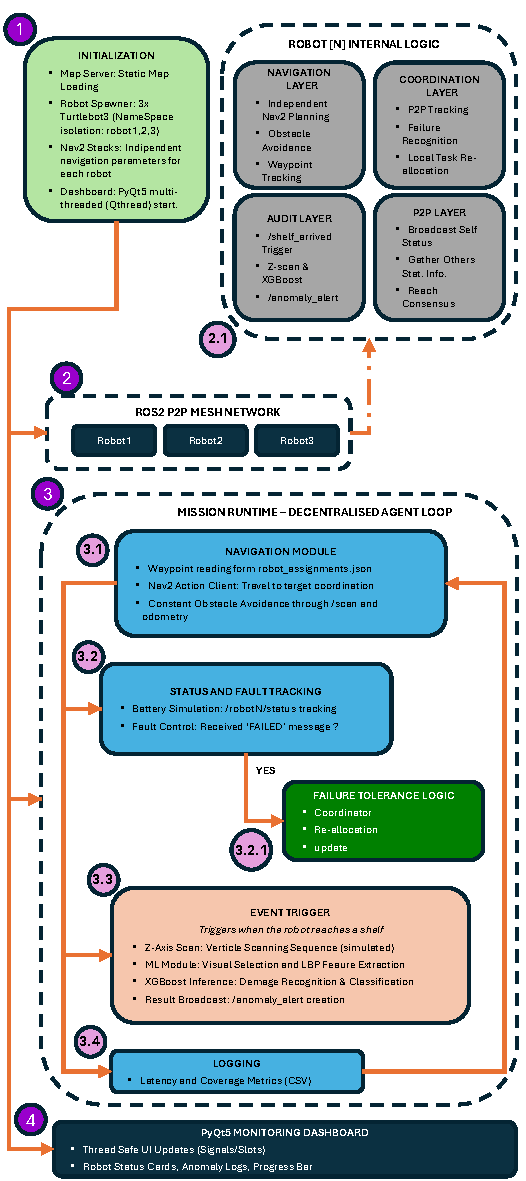
\includegraphics[width=0.96\linewidth, height=0.80\textheight]{Figures/Decentralized_Application_Workflow.pdf}
  \vspace{6pt}
  \captionof{figure}{\textbf{Decentralized Application Workflow:} \\ This diagram shows the data flow and decision mechanisms in the runtime of the simulation.}
  \label{Fig:Figure_1}
\end{figure}

\subsection{Multi-Agent Coordination and Job Distribution Mechanism}

The basis of the system is a fault-tolerant coordination procedure that does not need a central control unit. Every agent is going to be designed to communicate their status information and job progress through the system. In the case of an agent failure (fail scenario), it is planned to distribute the incomplete jobs (waypoint list) among active agents in a load-balanced way. This mechanism aims to achieve operational continuity by removing the risk of Single Point Failure (SPOF) and enables to analyze the effect of the count of agents (scalability) on total audit time.

\subsection{Navigation and Mapping Infrastructure}

Methodologically, the Nav2 stack and Cartographer SLAM will be integrated for robot navigation and mapping. Route planning, obstacle avoidance and target tracing processes are going to be carried out through each robot's costmaps. The Cartographer SLAM algorithm is preferred for environment mapping. In order for the robots to move safely and autonomously in the simulation environment, the Nav2 (Navigation 2) stack will be employed. In order to sensitively map wide areas at the scale of a warehouse, the LIDAR range is going to be increased to 20 meters in the simulation parameters and, through odometry data optimization, a static map is going to be achieved.

\subsection{Inventory Anomaly Detection System} 

To identify damaged packages in the inventory, an XGBoost machine learning algorithm will be used together with numerical feature extraction methods such as Local Binary Patterns (LBP). This model will be implemented, which is trained on using the "Defects in Cardboard Boxes" dataset sourced from Kaggle and Roboflow\cite{sarbeswar2024cardboarddefects}\cite{defects-1gsgd_dataset}.

\begin{enumerate}

    \item \textbf{Feature Extraction} - Numerical feature vectors will be generated from image data using Local Binary Patterns (LBP) and texture descriptors.

    \item \textbf{Integration} - In each shelf visit of the robots, a triggered ROS2 node will send the instant camera data by processing it and report the detected anomalies to the system with low latency. Model success is going to be validated through accuracy, precision and recall metrics. 

\end{enumerate}

\subsection{User Interface and System Monitoring Structure}

To improve operator awareness and real-time tracking of the system performance, a PyQt5-based multithreaded user interface is going to be developed. In order for the interface not to intervene, the ROS2 communication traffic data listening processes are going to be separated from the main interface loop via QThread structures. Through the panel, robots' real-time positions, job completion percentages, battery simulations and failure notifications that come from $/anomaly_alert$ topic will be visualized.

\vspace{10pt}
\subsection{Experiment Evaluation And Success Metrics}
\vspace{10pt}
System performance will be tested through 1, 2 and 3 agent scenarios by injecting controlled failures. The following metrics will be based on evaluation:
\vspace{10pt}
\begin{enumerate}
    \item \textbf{System Recovery Latency} - Time between the instant of failure and job redistribution.
\vspace{10pt}
    \item \textbf{Job Completion Efficiency} - Optimisation rate of total warehouse audit time under different agent counts.
\vspace{10pt}
    \item \textbf{Anomaly Detection Certainty} - Success of classification of the XGBoost model on real-time data.
\vspace{10pt}
    \item \textbf{Coverage Analysis} - Validation of any scanned shelf areas during the post-failure handover. 

\end{enumerate}


\begin{figure}[t]
  \centering
  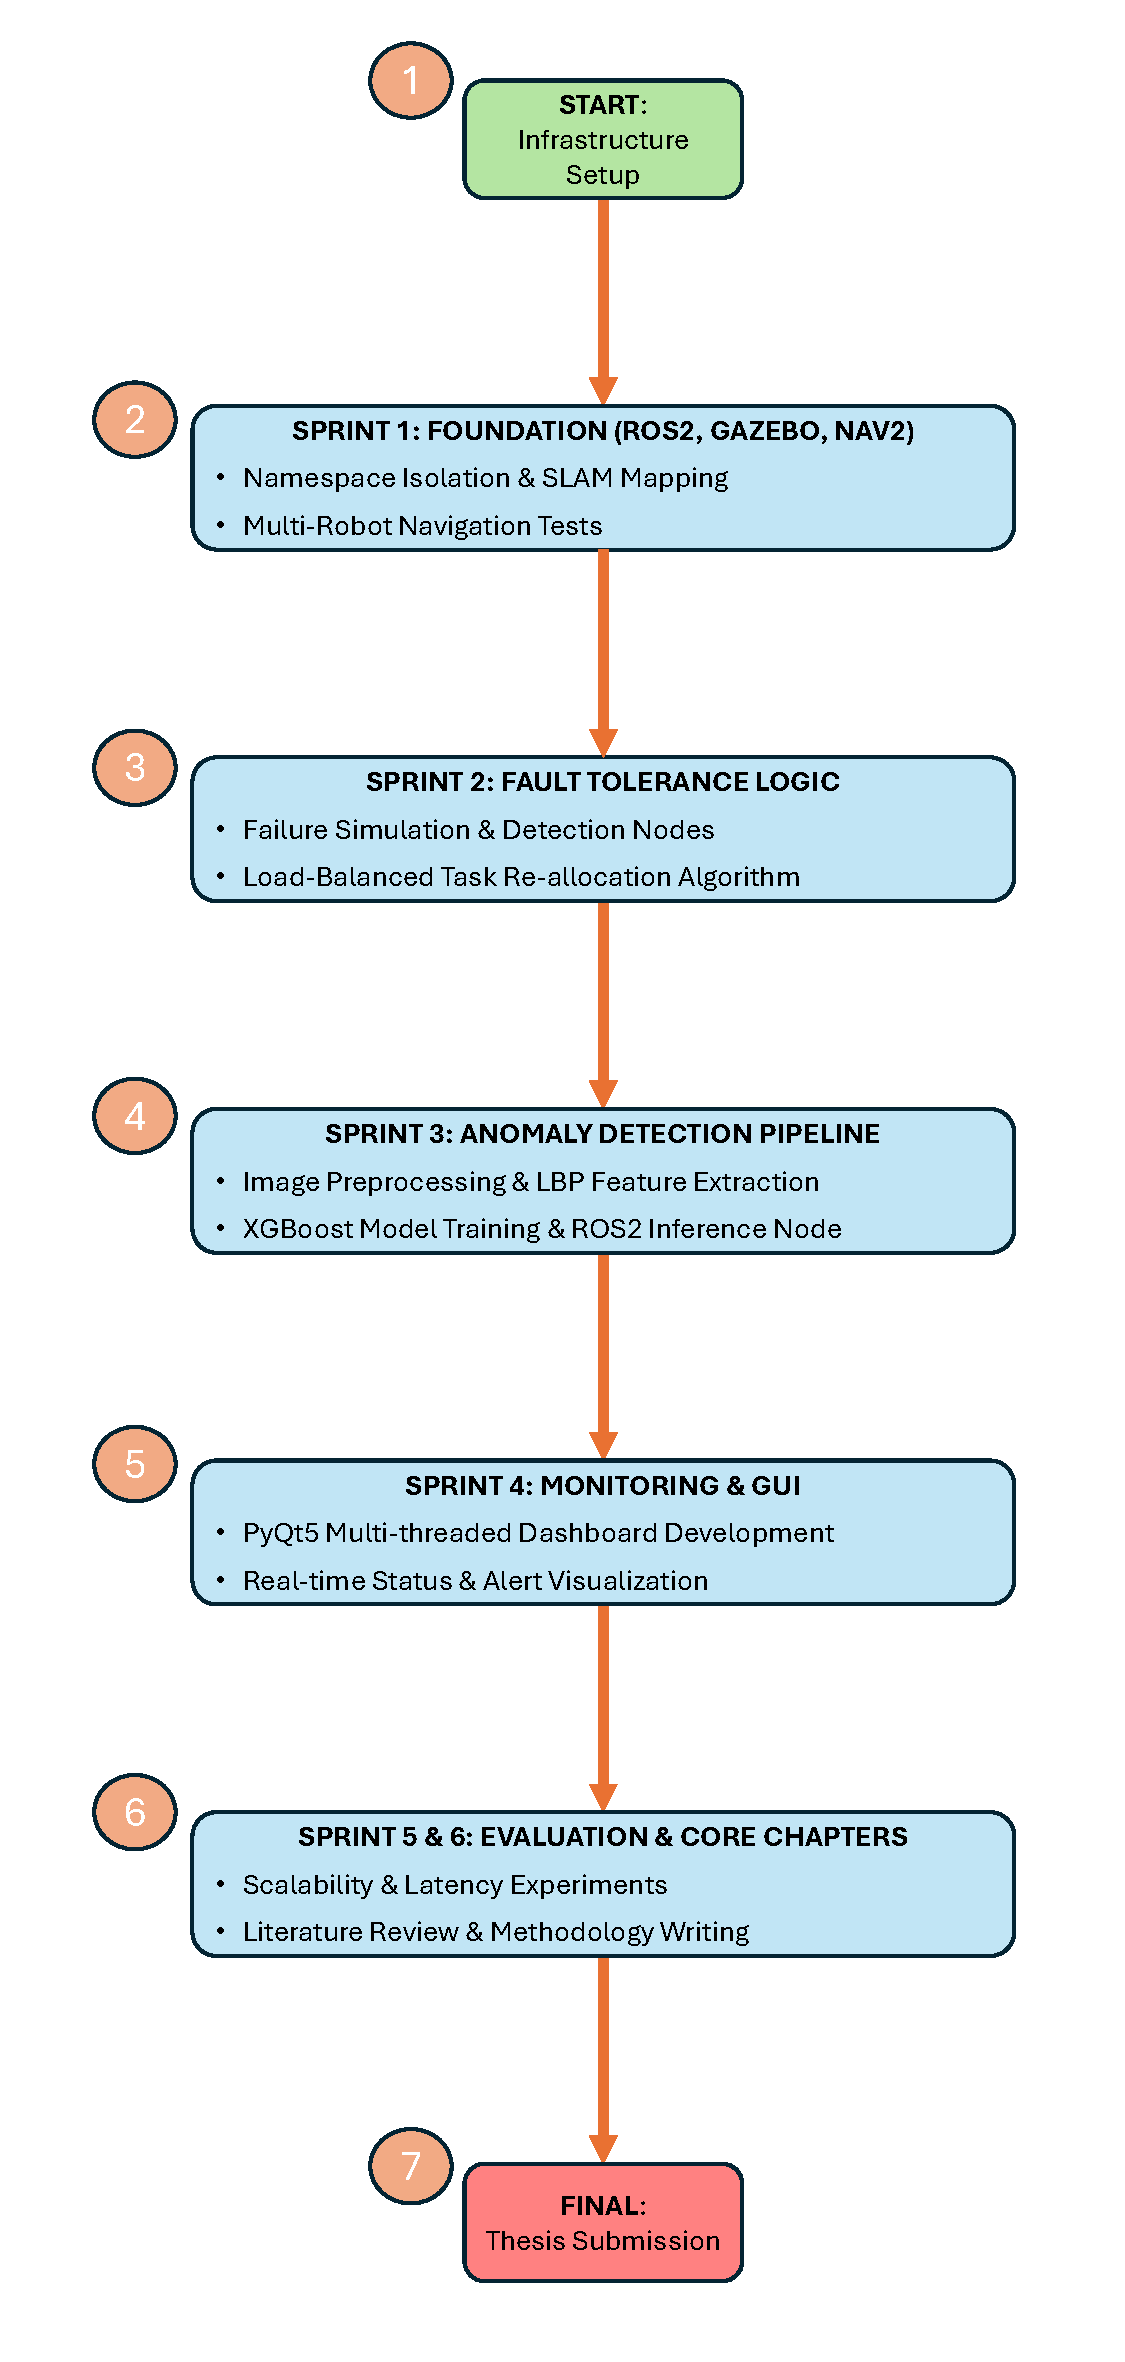
\includegraphics[width=\linewidth, height=0.75\textheight, keepaspectratio=true]{Figures/Project_Workflow.pdf}
  \vspace{5pt}
  \captionof{figure}{\textbf{Project Workflow:} \\
  Represents the workflow of the thesis project, starting from the initial design and development phases to the final evaluation and writing stages. Each sprint is designed to build upon the previous one, ensuring a structured and efficient progression towards the research objectives. Task breakdown and timeline are visualized in the Gantt chart in the Timeline section \ref{Fig:Figure_3}.}
  \label{Fig:Figure_2}
\end{figure}


\section{Expected Outcomes}

The primary outcomes and solutions to the industrial and academic problems that are expected to be achieved by this research are presented below:

\begin{itemize}
    
    \item \textbf{Decentralized and Fault-Tolerant Coordination Architecture} - The primary deliverable of this study is a ROS2-based autonomous multi-robot coordination framework that does not require a centralized control unit. This architecture, by eliminating the Single Point of Failure (SPOF) frequently emphasized in the literature, will ensure the system maintains operational continuity without crashing even in the event of an agent failure\cite{chandran2024network}.
    
    \item \textbf{Load-Balanced Dynamic Task Reallocation Algorithm} - A key technical output is the development of an algorithm for the redistribution of incomplete tasks (waypoints) among active robots. By optimizing the operational load in the event of agent attrition, this outcome directly minimizes downtime in warehouse operations and enhances total audit efficiency\cite{miele2025distributed}.
    
    \item \textbf{High-Precision Inventory Anomaly Detection Model} - The proposed XGBoost-based model is expected to provide low latency and high classification accuracy for identifying damaged packages. By reducing human error in manual audit processes, this outcome will significantly improve inventory visibility and data reliability\cite{arvind2025intelligent}.
    
    \item \textbf{Feasibility and Simulation Fidelity} - The technical stack employed (ROS2 Jazzy, Gazebo Harmonic, and Turtlebot3 Waffle) consists of proven tools for warehouse automation scenarios\cite{leite2024coordination}. The simulation environment, supported by NVIDIA GPU hardware acceleration and MESA D3D12 drivers, provides high fidelity through realistic physical engine capabilities and sensor data, strengthening the transferability of the results to real-world applications.
    
    \item \textbf{Interdisciplinary Value and Industry 5.0 Vision} - This project integrates software engineering (distributed systems), robotics (autonomous navigation), and artificial intelligence (anomaly detection).     
\end{itemize}

The outcomes will contribute not only to the logistics sector but also to other fault-critical multi-agent operations, such as search and rescue and environmental monitoring, providing significant interdisciplinary value.


\bibliographystyle{IEEEtran}

\bibliography{Bibliography}


\clearpage
\onecolumn
\section{Timeline}

\begin{figure}[H]
    \centering
    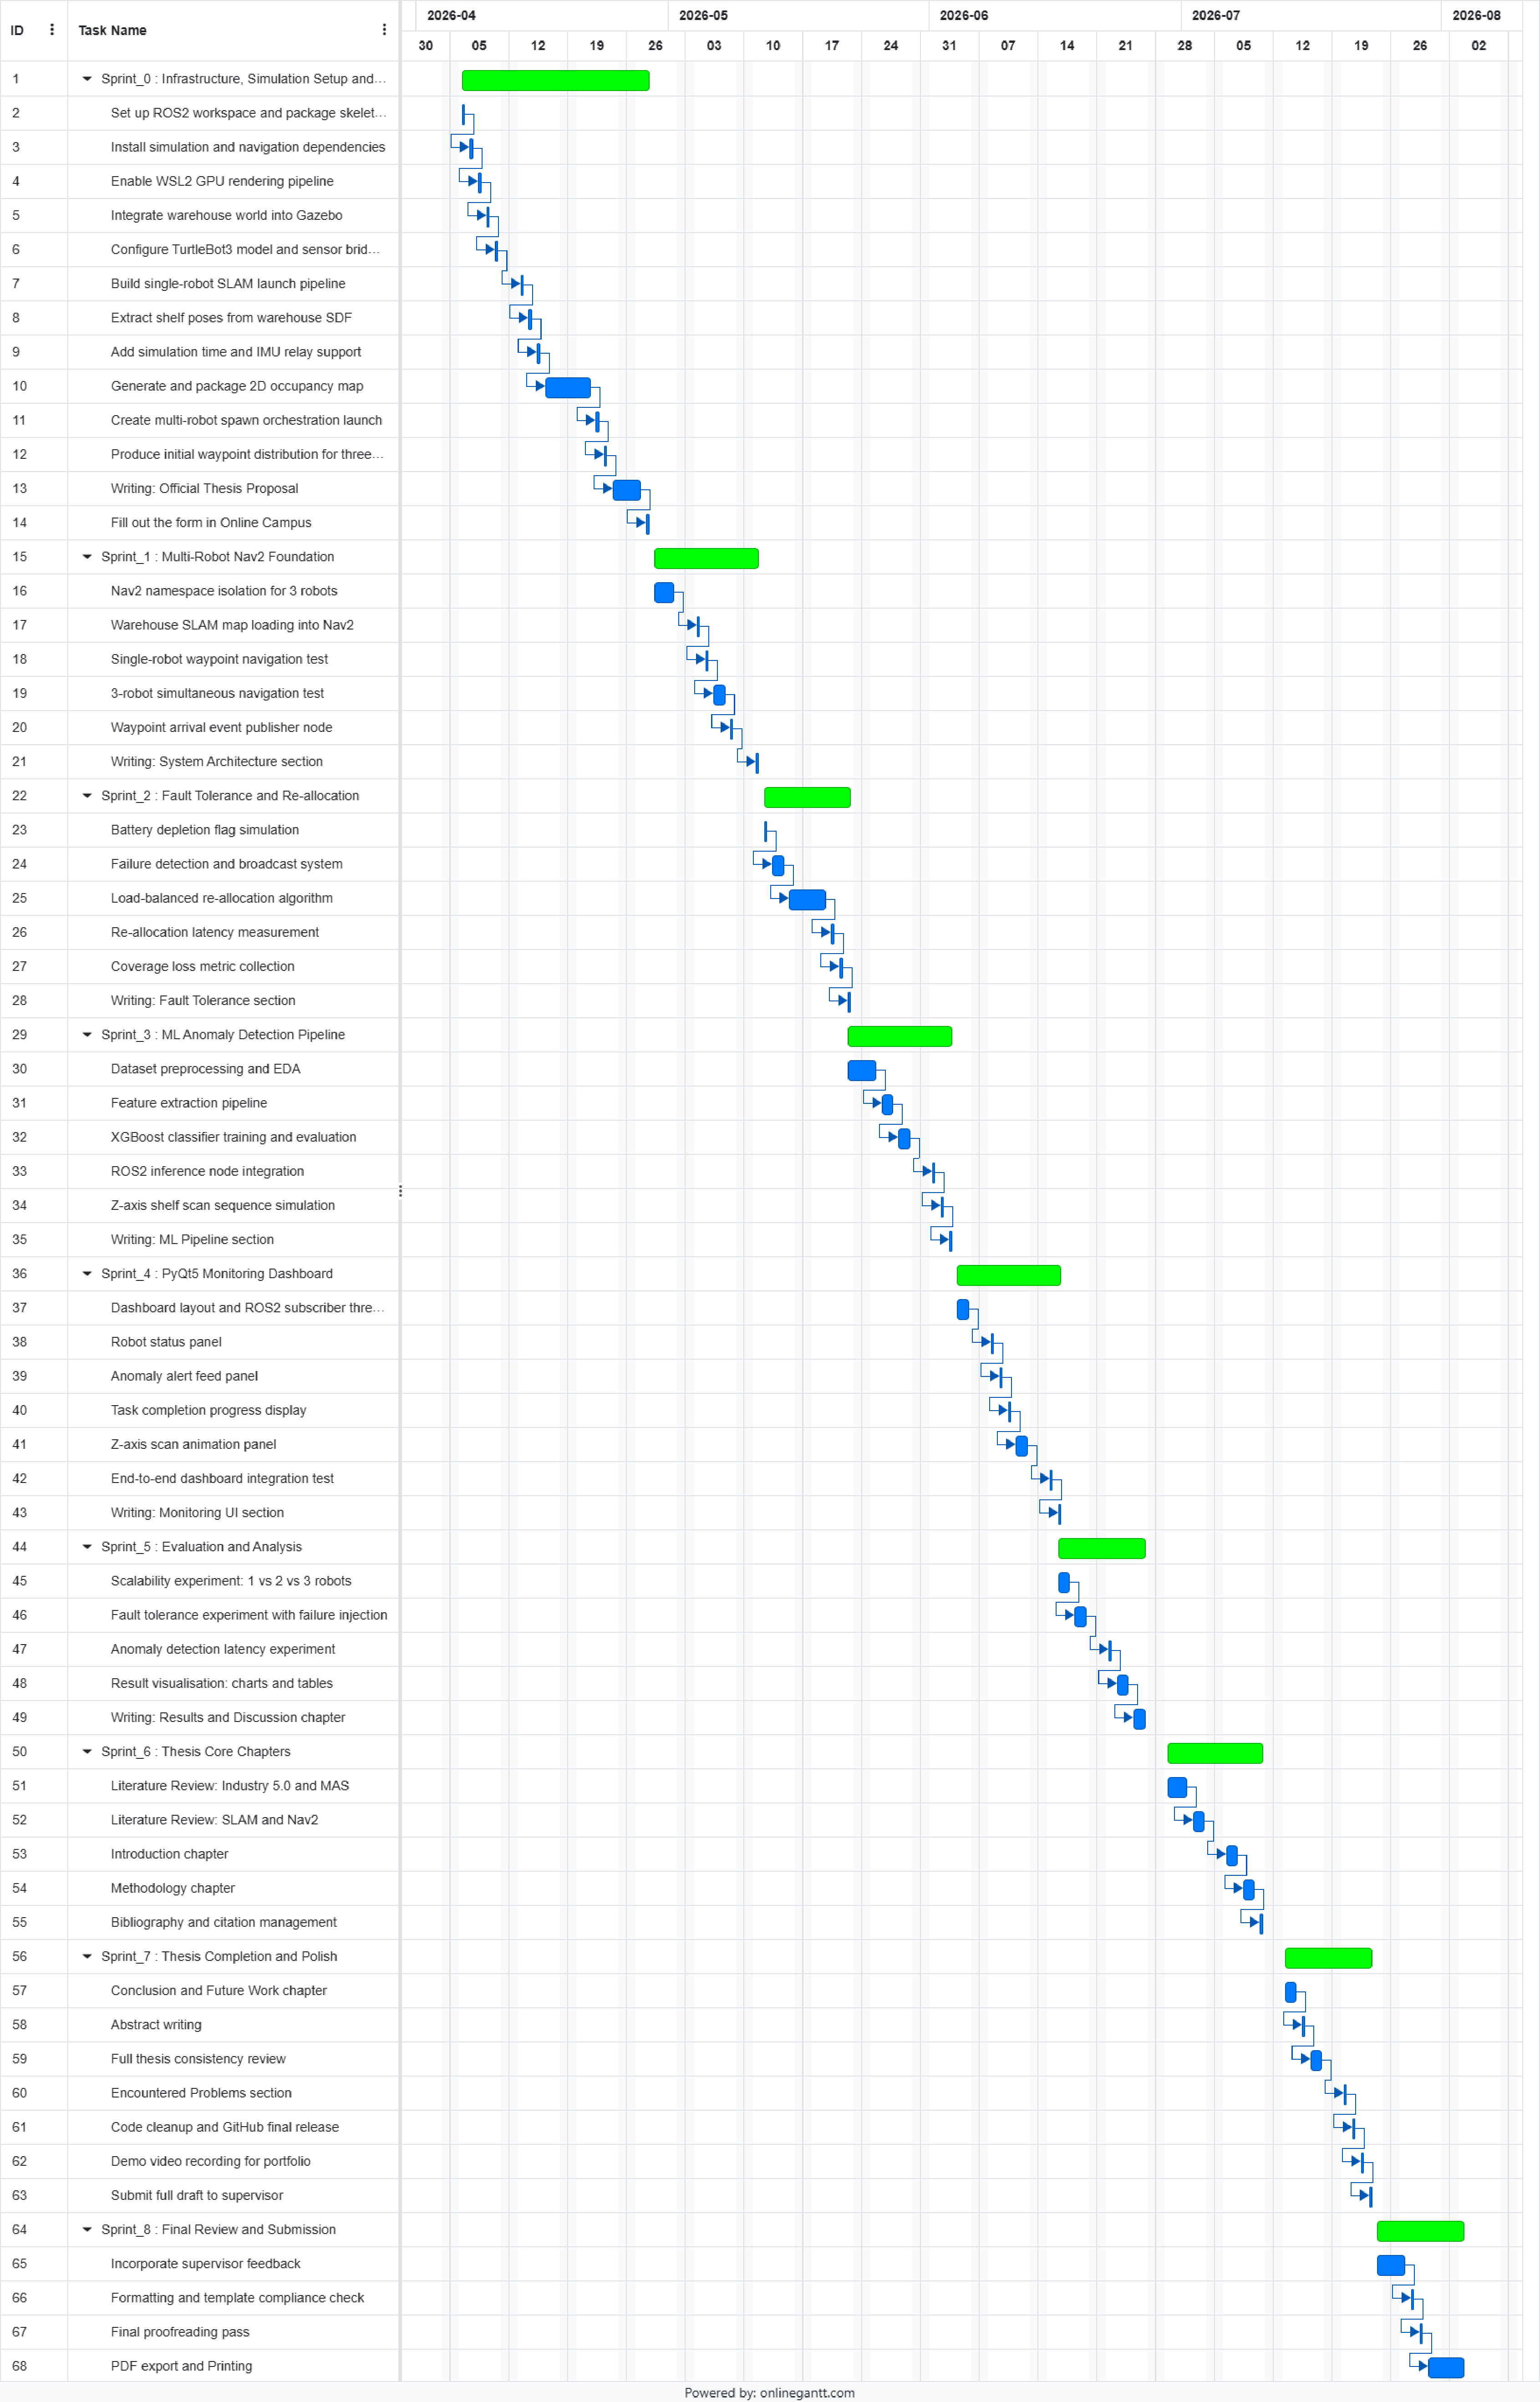
\includegraphics[width=\textwidth, height=0.9\textheight, keepaspectratio=true]{Figures/gantt_chart.pdf}
    \vspace{8pt}
    \caption{The thesis project building, result evaluation and result writing processes have been broken into 9 sprints and each sprint has been divided into successive tasks as presented in the Gantt Chart.}
    \label{Fig:Figure_3}
\end{figure}


  \end{document}
